\documentclass[12pt, letterpaper]{article}
\usepackage{graphicx}

\title{Visualization of website publish date frequency using htmldate python package}
\author{Raufir Ahmed Shanto}
\date{August 6, 2020}

\begin{document}

\maketitle

\section{Introduction}

Metadata extraction is part of data mining and knowledge extraction. Being able to better
qualify content allows for insights based on descriptive or typological information (e.g., content
type, authors, categories), better bandwidth control (e.g., by knowing when webpages
have been updated), or optimization of indexing (e.g., caches, language-based heuristics). It
is useful for applications including database management, business intelligence, or data visualization.
This particular effort is part of a methodological approach to derive information
from web documents in order to build text databases for research, chiefly linguistics and natural
language processing. Dates are critical components since they are relevant both from a
philological standpoint and in the context of information technology.

 
In this project, I have used this htmldate \footnote{https://github.com/adbar/htmldate} package to extract publication date for most popular 500 websites. Then I have written a python program which creates two histogram plots.

\section{Dataset}


I have collected the dataset from https://moz.com/top-500/download/?table=top500Domains which is a CSV file and saved as top500Domains.CSV. Upon opening the dataset, I have got to know that this dataset has following variable:

\begin{table}[h]
\begin{tabular}{|l|l|}
\hline
Variable & Description and units                                                      \\ \hline
\texttt{Rank}    & Rank of the website according to the DA ranking                          \\
\texttt{Root Domain}     & Domain Name                                                \\
\texttt{Linking Root Domains}    &  The number of other sites that link to that page        \\
\texttt{Domain Authority}    & Search Engine Ranking                                                      \\
              \\ \hline
\end{tabular}
\caption{Variables in Moz data}

\end{table}

My point of interest in the dataset was Domain Name column. The prefix "https://" was required to call the find\_date() function. Therefore, I have written a program named web\_publish\_date.py which takes the dataset as input, sanitizes it, finds publish date of the domain's and puts it's it into a new column in the dataframe.


To quantify whether SST for a particular area is indeed abnormally warm, we will use the Marine Heatwave (MHW) definition of Hobday et al. (manuscript submitted to Progress in Oceanography).  An algorithm for detecting a MHW has been implemented in the Python package `marineHeatWave`.

\section{Results}

I have visualized the publish date of domains in two plots. One of them is publish date vs year timeline another is publish date vs month timeline. The results were generated using matplotlib library of python.


\begin{figure}
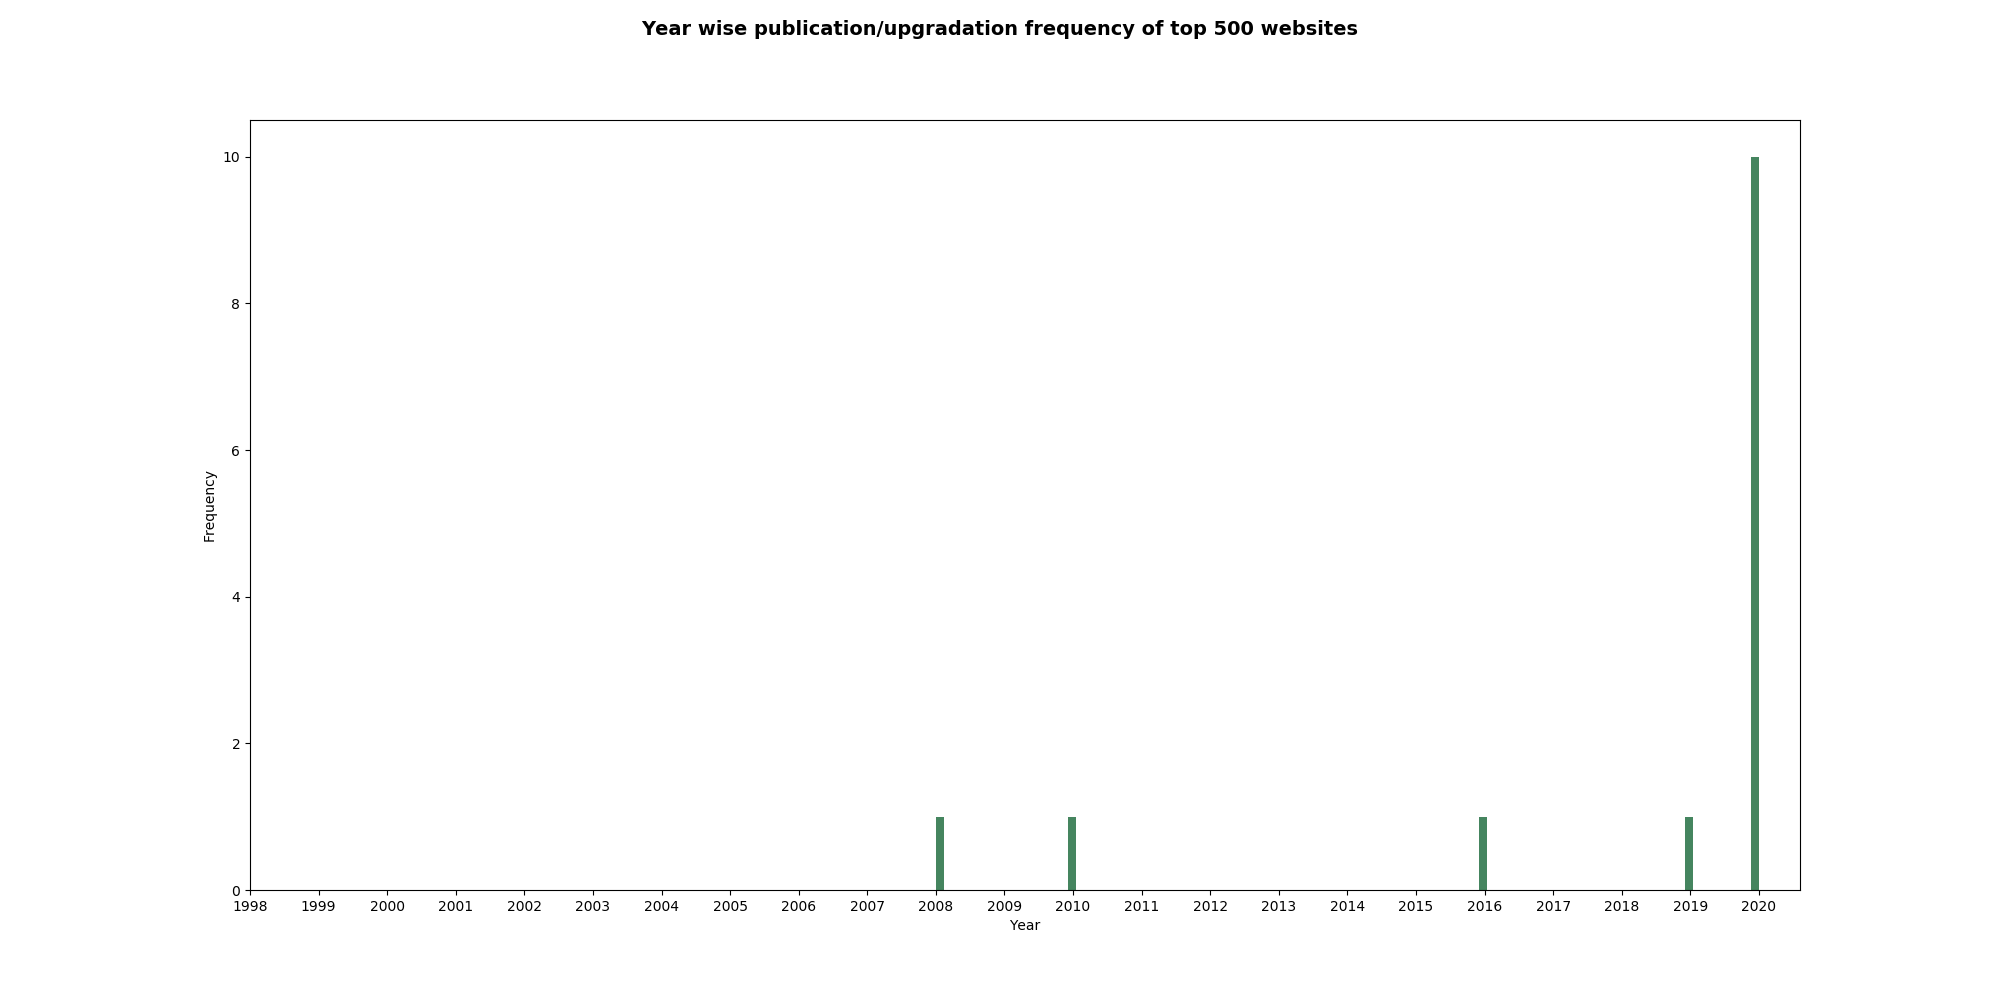
\includegraphics[width=0.9\textwidth]{Plot1.png}
\caption{Website publish/upgrade date in yearly timeline}
\label{fig:plot1}
\end{figure}

\begin{figure}
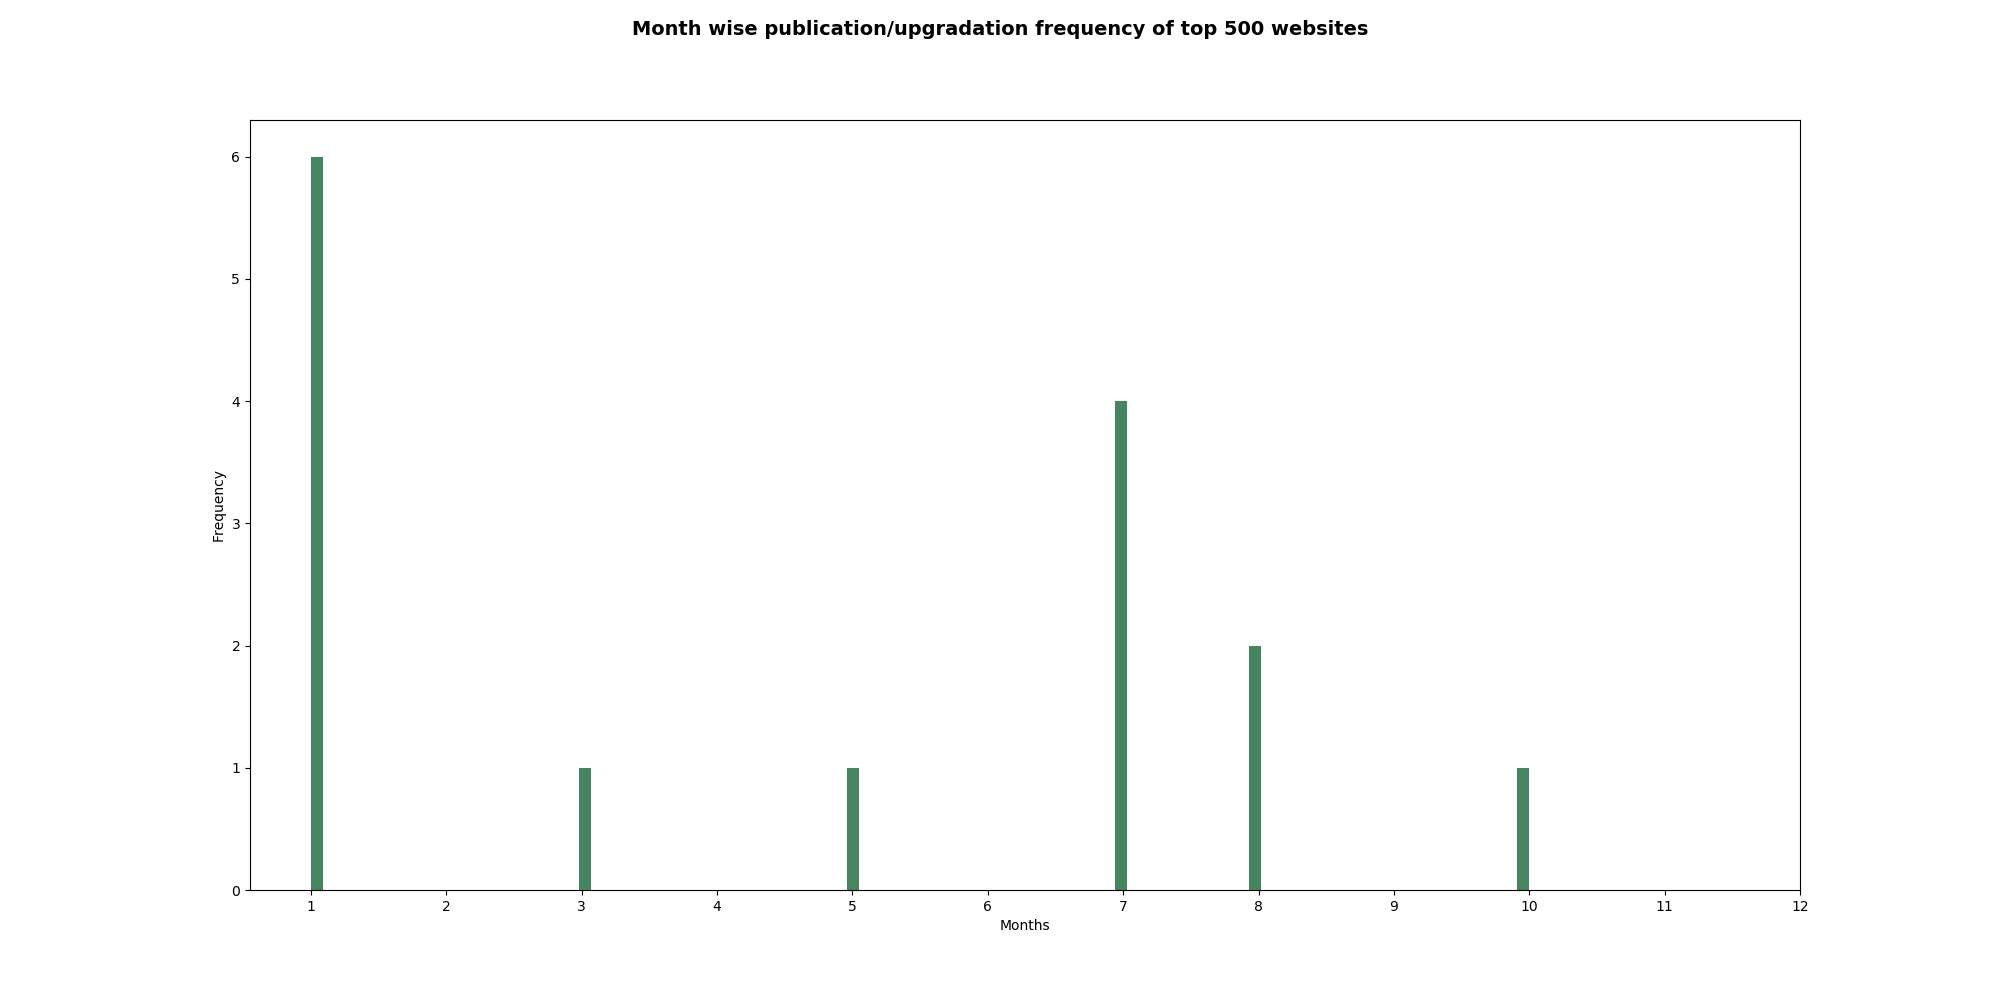
\includegraphics[width=0.9\textwidth]{Plot2.png}
\caption{Website publish/upgrade date in monthly timeline}
\label{fig:plot2}
\end{figure}



\section{Conclusions}
From the results we can observe that, most of the popular websites are published or updated in year 2020. On a different perspective we can see that, most of the websites are published or updated in January or August.

% would be good to a a bibiography here too.

\end{document}
